\documentclass[conference]{IEEEtran}
\pdfpagewidth=8.5in
\pdfpageheight=11in
%\usepackage{subfig}
%\usepackage{subfigure}
\usepackage[pdftex]{}
\usepackage{graphicx}
%\usepackage{todonotes}
\usepackage{listings}
\lstset {% general command to set parameter(s)
         language=C,
     basicstyle=\footnotesize,               % print whole listing small
%     keywordstyle=\color{black}\bfseries, % underlined bold black keywords
%     identifierstyle =\color{black},  % nothing happens
%     commentstyle=\color{black}\emph, % white comments
     %stringstyle=\ttfamily,          % typewriter type for strings
%     stringstyle=\color{black},       % typewriter type for strings
         tabsize=4,
         showtabs=false,
     showstringspaces=false}
%can't figure this one out for particles bandwidth
%\usepackage[caption,label]{subfig}

%\newcommand{\TITLE}{D\textsuperscript{\huge{2}}T: Doubly Distributed Transactions for High Performance and Distributed Computing}

\newcommand{\DDT}{D\textsuperscript{2}T~}
\newcommand{\DDTns}{D\textsuperscript{2}T}

\hyphenation{sub-trans-ac-tion}

\addtolength{\parskip}{-0.06in}

% in order for balance columns to work, it has to be before begin document...
%\balancecolumns

\begin{document}

%\conferenceinfo{Cluster'14,} {September 17, 2014, Madrid, Spain}
%\CopyrightYear{2014}
%\crdata{978-1-4503-1103-8/11/11}
%\clubpenalty=10000
%\widowpenalty = 10000

\title{An Innovative Storage Stack Addressing Extreme Scale Platforms and Big Data Applications}

\author{
\IEEEauthorblockN{Jay Lofstead\IEEEauthorrefmark{1}, Ivo Jimenez\IEEEauthorrefmark{2}, Carlos Maltzahn\IEEEauthorrefmark{2}, Quincey Koziol\IEEEauthorrefmark{3}, John Bent\IEEEauthorrefmark{4}, Eric Barton\IEEEauthorrefmark{5}}
\IEEEauthorblockA{\IEEEauthorrefmark{1}Sandia National Laboratories gflofst@sandia.gov}
\IEEEauthorblockA{\IEEEauthorrefmark{2}University of California, Santa Cruz ivo@cs.ucsc.edu, carlosm@soe.ucsc.edu}
\IEEEauthorblockA{\IEEEauthorrefmark{3}HDF Group koziol@hdfgroup.org}
\IEEEauthorblockA{\IEEEauthorrefmark{4}EMC john.bent@emc.com}
\IEEEauthorblockA{\IEEEauthorrefmark{5}Intel eric.barton@intel.com}
}
\maketitle

\begin{abstract}
The DOE Extreme-Scale Technology Acceleration Fast Forward Storage and IO Stack
project is going to have significant impact on storage systems design within
and beyond the HPC community. With phase 1 of the project complete, it is an
excellent opportunity to explore the complete design and how it will address
the needs of extreme scale platforms.  This paper not only provides a timely
summary of important aspects of the design specifications but also capture the
underlying reasoning that is not available elsewhere. With this information, we
encourate the broader community to understand the design, intent, and future
directions to foster discussion guiding phase 2 and the ultimate production
storage stack based on this work.

While many of the design elements are best practices from current research,
there are many new contributions as well as different integration approaches
offering different performance and quality of service guarantees. The specifics
of how the different layers interact offer a new approach for managing data for
extreme scale platforms and workloads.

For the current demonstration system, the HDF5 user API gives a familiar
way to interact with all of the new functionality while largely insulating 
end-users from the intracisies of dealing with the advanced functionality
offered by the stack.  The various layers below the user API include optional
components that may aid in scalability and simplify implementation across a
wide range of platforms.  The data storage layer offers support both
for local machine and data center wide storage arrays as part of the design.

In addition to these features supporting HPC platforms, the stack also
addresses the need of big data applications as demonstrated through the
Arbitrary Connected Graphs tool.

\end{abstract}

%\category{D.4}{Software}{Operating Systems}
%\category{D.4.7}{Operating Systems}{Organization and Design}[hierarchical design]

%\terms{Design, Performance}

\section{Introduction}

Current production HPC IO stack design is unlikely to offer sufficient features
and performance to adequately serve the needs of an extreme scale platform.
Adding to the complexity of the problem is the variety of Big Data problems
that are taking advantage of these platforms. Trying to address both of these
domains is a daunting problem.

To address these challenges, a joint effort between the US Department of
Energy's Office of Advanced Simulation and Computing and Advanced Scientific
Computing Research commissioned an effort to develop a design and prototype for
an IO stack suitable for the extreme scale environment called the Fast Forward
Storage and IO (FFSIO) project. This is a joint effort led by Lawrence
Livermore National Laboratory, with the DOE Data Management Nexus leads Rob
Ross and Gary Grider as coordinators and contract lead Mark Gary. The
participating labs are LLNL, SNL, LANL, ORNL, PNL, LBNL, and ANL.  Additional
industrial partners contracted include the Intel Lustre team, EMC, DDN, and the
HDF Group. This team has developed a specification
set~\cite{fastforward:2014:docs} for a future IO stack to address the
identified challenges. The first phase recently completed with a second phase
currently getting underway as of early 2014. The core focus of the first phase
was basic functionality and design. While an idealized potential system would
be the perfect target architecture, the reality of budgets has tempered many of
the decisions. For exmaple, extensive availability of NVRAN or SSDs on all of
the compute nodes is currently not economically feasible limiting some of the
potential design choices.  With this in mind, the second phase will refine this
design incorporating fault recovery and other features missing from the first
phase.

The complete design seeks to offer high availability, byte-granular,
multi-version concurrency control. Through the use of a copy-on-write style
mechanism reducing space and time requirements, multiple versions of an object
can be stored efficiently. By assuming the client interface will be through an
IO library, a more complicated interface that offers richer functionality can
be incorporated while requiring only minimal end-user code changes.  Managing
most data access in a platform-local layer rather than requiring writing to
centralized storage will better support the performance and energy requirements
of extreme scale integrated application workflows.

Overall, the architecture shifts from the idea of files and directories to
containers of objects. This shift avoids the bottlenecks related to the POSIX
files and directories structure such as the serialization of file creation, the
limitation and impact of the number of files in a directory, and the limited
semantics of a byte stream. Instead, the new interface focuses on high-level
data models and their properties and relationships. This concept permeates the
entire IO stack.

In addition to addressing the traditional scientific workload, this project
seeks to expand functionality to better support Big Data type applications. The
key idea is to support Arbitrary Connected Graphs (ACGs) such as those used in
Map-Reduce systems. Key system features are introduced to efficiently support
these computing models in addition to the typically bursty IO loads of more
traditional HPC applications.

\begin{figure}[htbp]
\centering
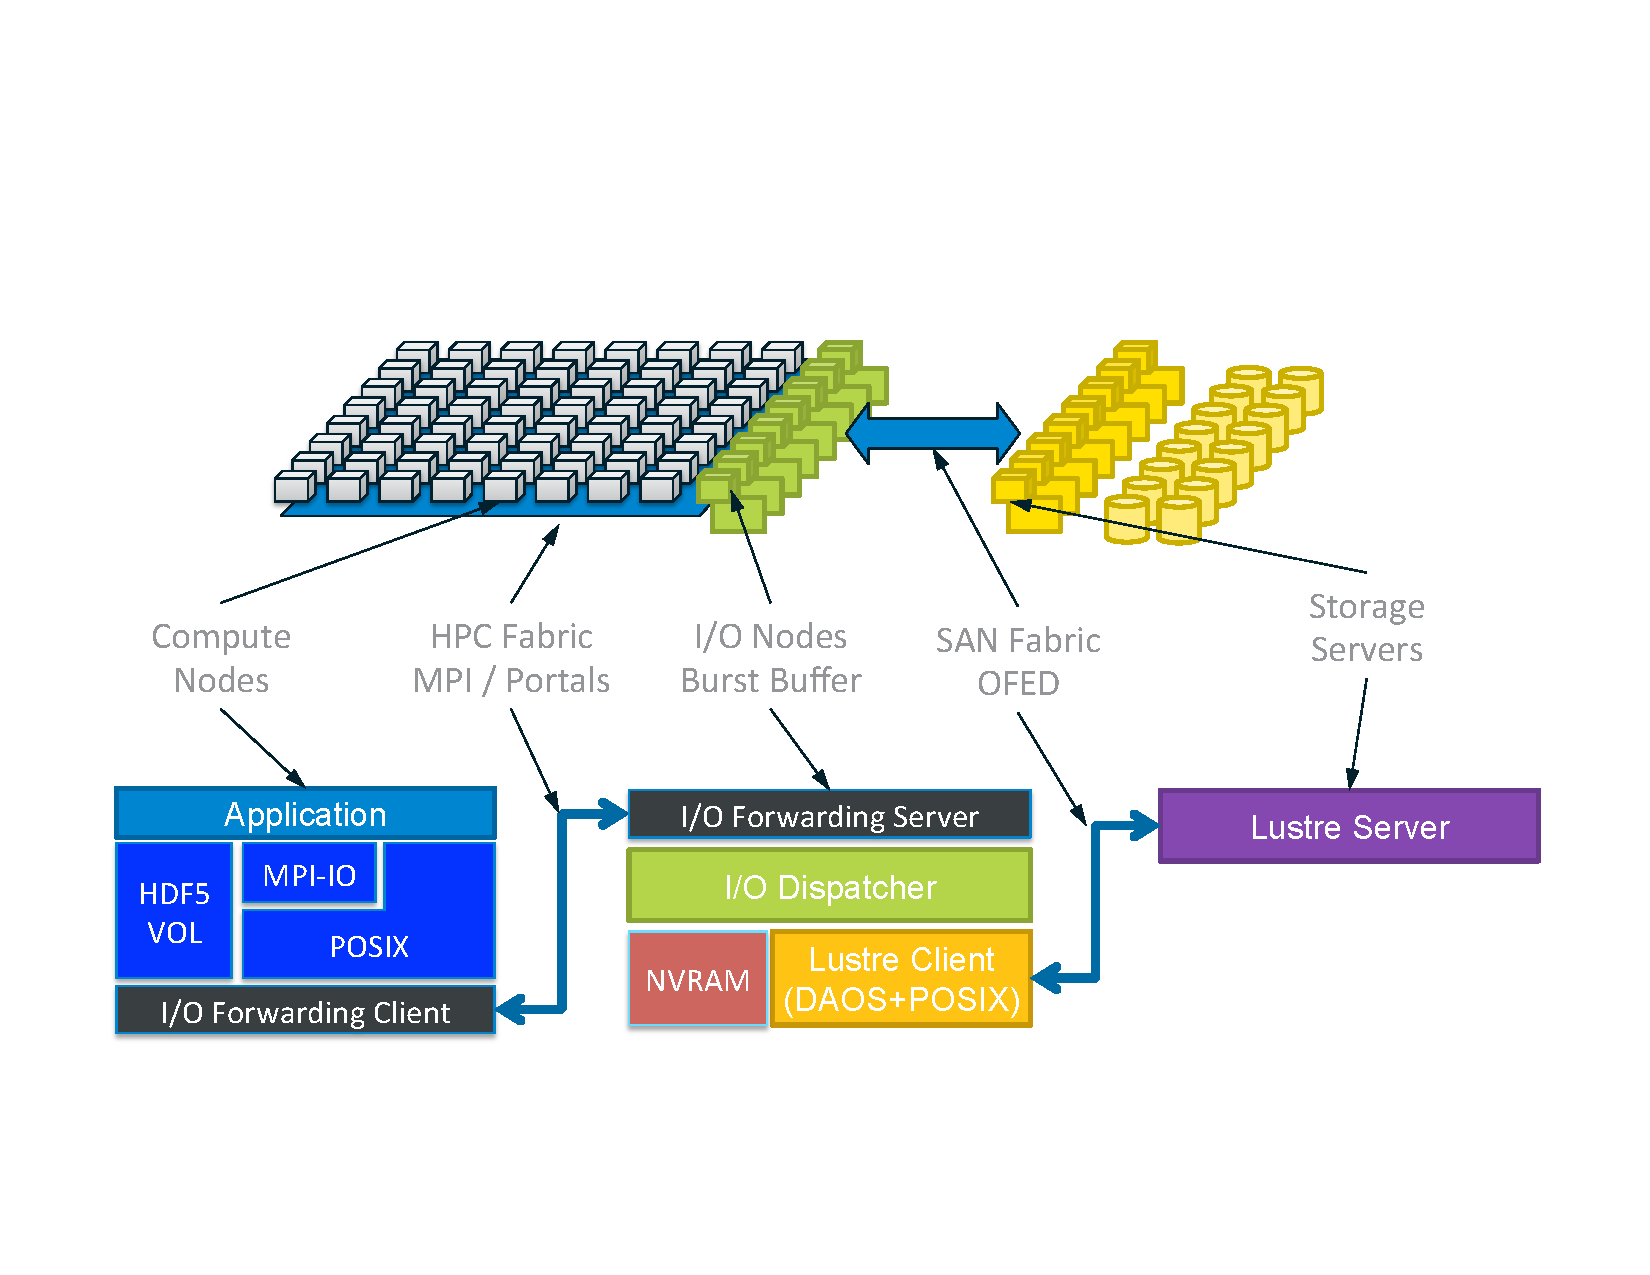
\includegraphics[width=\columnwidth]{images/arch-mapping}
\caption{Target Architecture and Component Mapping}
\label{fig:arch-mapping}
\end{figure}

At a more detailed view, the various layers of the IO stack each contribute
different functionality and performance implications.  The
architecture (Figure~\ref{fig:arch-mapping}) incorporates five layers, some of
which have potentially optional components.  The top layer is generally a high
level IO library, such as the demonstration HDF-5 library~\cite{hdf5}. It is in
dark blue. The intent is to only have access to the storage stack through such
an API to manage the complexity of working with the lower layers and to enable
advanced functionality that would require more direct user intervention. This
layer incorporate the necessary features for ACGs from a end-user's
perspective.

Below the user API is an IO forwarding layer that redirects IO calls from the
compute nodes to the IO dispatching layer (in black).  This IO forwarding layer
is analogous to the function of the IO nodes in a BlueGene machine or the
passive data staging processes demonstrated
previously~\cite{nisar:2008:staging,Abbasi:2009:datatap}. The next two layers
have considerable functionality. The IO dispatcher (IOD) serves as the primary
storage interface for the IO stack and is the only way to reach the persistent
storage array in lower layers (in green). Ideally, the IOD layer's
functionality can be optional based on available hardware. Much of the
functionality offered at this layer would shift either up or down the stack as
discussed in detail below. The Distributed Asynchronous Object Storage (DAOS)
layer serves as the persistent storage interface and is intended to be the
traditional file system-like foundation on which everything else is built with
no dependence on any technologies specified above it (in pink and yellow). For
example, the IOD layer with or without burst buffers is not required for DAOS
to operate properly.  Instead, the DAOS layer can handle all of the IO
operations from the user API layer, albiet with the potential performance
penalty of manipulating the shared, persistent storage array. At the bottom is
the Versioning Object Storage Device (VOSD) (in purple).  It serves as the
interface for storing objects of all types efficiently. Think of this layer as
the physical disk interface layer. In terms of Lustre, this would replace the
file system on individual storage targets with an interface friendlier to the
containers of objects concept used in the higher layers.

Along with the analysis of the published design documents, a discussion of the
design philosophy representing the overall intent is presented. This
information represents information that may or may not have been written down,
but is the intent of ultimate product.  These ideas are presented to give a
fuller picture of where the project is going rather than dwelling on any
limitations of the published documents.

The rest of the paper is organized as follows. A brief overview of related work
is presented first in Section~\ref{sec:related}. Section~\ref{sec:end-user}
discusses the programmatic interface end users will see when interacting with
the storage array. This will be discussed in the contect of the HDF-5 based
example library used for the functionality demonstration. Section~\ref{sec:iof}
briefly discusses the motivation and proposal for the IO forwarding layer.
Section~\ref{sec:iod} describes the IO Dispatcher layer and the broad
functionality it offers. This will detail the pieces of the layer that are
potentially optional and mention the cross-cutting features discussed in a
later, cross-cutting section. Section~\ref{sec:daos} discusses how the
persistent storage array interface itself functions. As with the IOD layer, the
disucssion of cross-cutting features will be mentioned, but disucssed more
fully in the cross-cutting section. The VOSD layer is disucssed in
Section~\ref{sec:vosd}. In particular, the mapping between the DAOS and VOSD
layers are explored as it pertains to the physical storage. Next is an
exploration of cross-cutting features like transactions and metadata management
in Section~\ref{sec:broader}. Since these and other features are spread across
multiple layers, it makes more sense to discuss them independently once an
understanding of the overall structure has been presented.  A demonstration
of the functionality is presented in Section~\ref{sec:evaluation}. This shows
that the prototype functionality validation prototype can function. The paper
is concluded in Section~\ref{sec:conclusion} with a summary of the broad issues
covered in the paper.

\section{Related Work}
\label{sec:related}

Many projects over the last couple of decades have sought to address some
challenging aspect of parallel file system design. The recent rise of the ``Big
Data'' applications with different characteristic IO patterns have somewhat
complicated the picture. Extreme scale machines will be expected to handle both
the traditional simulation-related workloads as well as applications more
squarely in the Big Data arena. This will require some adjustments to the
underlying system for good performance for both scenarios.

The major previous work is really limited to full file systems rather than the
mountain of file system adjustments made over the years.

Ceph~\cite{weil:ceph} is a distributed object store and file system. It offers
both a POSIX and object interface including features typically found in parallel
file systems. Ceph's unique striping approach uses pseudo-random numbers with a
known seed eliminating the need for the metadata service to track where each
stripe in a parallel file is placed.

PVFS~\cite{carns:pvfs} offers optimizations to reduce metadata server load,
such as a single process opening a file and sharing the handle.

Lustre~\cite{braam:lustre-arch} has become the defacto standard on most major
clusters offering scalable performance and fine-grained end-user and programmatic control over how data is placed in the storage system. Scalability limitations are part of the motivation for the FFSIO project.

GPFS~\cite{schmuck:gpfs} offers a hands-off approach for providing good performance for scaling parallel IO tasks and is used extensively by its owner, IBM.

Panasas~\cite{panasas:architecture} seeks to offer a dynamically adaptive striping system that detects the need for additional stripes for performance and adjusts the file layout as necessary.

Other file systems, like GoogleFS~\cite{ghemawat:googlefs}, address distributed
rather than parallel computing and cannot be compared directly. The primary
difference between distributed and parallel file systems is the ability of the
file system to retrieve data simultaneously from multiple clients, in parallel,
and treat the resulting collection of pieces as a single object. Distributed
file systems rely on a single client creating a file, but distributing the set
of files across a wide array of storage devices. The other, popular distributed
file system of note is HDFS~\cite{Shvachko:2010:hdfs} that is distributed as
part of Hadoop. These other file systems are mainly of interest in the context
of the ACG features of FFSIO and will be discussed more in
Section~\ref{sec:acg}.

\section{End-User API Layer}
\label{sec:end-user}
Since the proposal specifies a high-level IO API will be the primary end-user
interface for programmatically interacting with the FFSIO stack, the team used
the HDF-5 API and leverated the Virtual Object Layer (VOL) for the initial
design and implementation demonstration. The VOL provides a way to intercept
HDF-5 API calls just below the API layer to implement alternative
functionality. For this project, rather than the default writing to disk in the
HDF-5 format, the VOL layer is used to interact with the IOD layer and the new
concepts it offers, such as transactions, completely hidden from the user.
This both offers a straightforward way for existing applications to test
against the FFSIO stack and to ensure proper semantics are maintained at the
lower levels. Some additional API functions have been introduced to support
new functionality, such as the ACG support for Hadoop-style applications.  The
additions comprise (Figure~\ref{fig:vol-arch}):

\begin{enumerate}
\def\labelenumi{\arabic{enumi}.}
\itemsep1pt\parskip0pt\parsep0pt

\item
  Object-storage API based on HDF5 to support high-level data models.
  This exposes asynchronous, transactional semantics to the application,
  as well as end-to-end data integrity. It will also allows the usage of
  pointer data types, passing of hints down to the storage and support
  for asynchronous index building, maintenance and querying.

\item
  Virtual Object Layer (VOL) plugin that translates HDF5 API requests
  from applications to IOD API calls.

\item\label{item:fs}
  Function shipping from Compute Nodes (CN) to IO Nodes (ION). This provides
  the application developer with the capacity of sending computation down to the
  IONs and get back results.

\item
  Analysis Shipping from CN to IONs or DAOS nodes. This is similar
  to~\ref{item:fs} but instead of returning the result over the network, it
  gets stored on the nodes and pointers to it are returned.

\end{enumerate}

Function and Analysis Shipping are part of the cross-cutting features and are
discussed in Section~\ref{sec:fn-shipping}.

HDF5~\cite{hdf5} is a versatile data model containing complex data objects
and metadata. Its information set is a collection of datasets, groups,
datatypes and metadata objects. The data model defines mechanisms for
creating associations between various information items. The main
components of HDF5 are described below.

\begin{figure}[htbp]
\centering
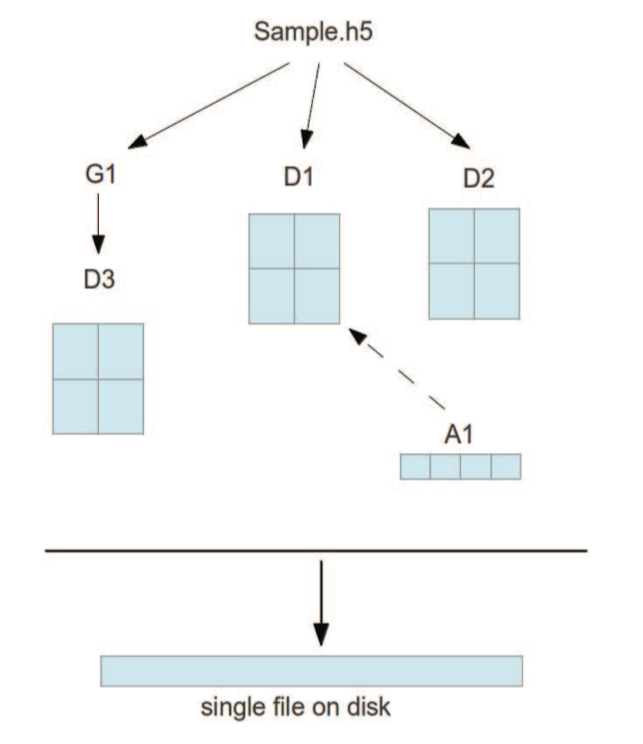
\includegraphics[scale=0.30]{images/hdf5.png}
\caption{Sample file illustrating the hierarchical structure of HDF5 files}
\label{fig:hdf5-sample}
\end{figure}

\begin{itemize}

\item
  \textbf{File}: In the HDF5 data model the container of an HDF5 infoset
  is represented by a file. It is a collection of objects that also
  explains the relationship between them. Every file begins with a root
  group ``/'', which serves as the ``starting-point'' in the object
  hierarchy.

\item
  \textbf{Dataset}: HDF5 datasets are objects that represent actual data
  or content. Datasets are arrays which can have multiple dimensions. A
  dataset is characterized by a dataspace and a datatype. The dataspace
  captures the rank (number of dimensions), and the current and maximum
  extent in each dimension. The datatype describes the type of its data
  elements.

\item
  \textbf{Group}: A group is an explicit association between HDF5
  objects. It is synonymous with directories in a file system. A group
  could contain multiple other groups, datasets or datatypes within it.

\item
  \textbf{Attribute}: Attributes are used for annotating datasets,
  groups, and datatype objects. They are datasets themselves, and are
  attached to existing objects they annotate.

\end{itemize}

For example, as shown in Figure \ref{fig:hdf5-sample}, the file Sample.h5
contains the root group which itself contains a group G1 and two datasets, D1
and D2. Group G1 contains a dataset D3. Attribute A1 is linked to dataset D1.
The objects and the relationships between them can be represented as a B-tree,
which is used internally by HDF5 to index its objects.

The Fast Forward project is working on the adaptation of the HDF5 libraries in
order to expose the storage stack to applications.

\subsection{Virtual Object Layer}
\label{virtual-object-layer}

The Virtual Object Layer is an abstraction mechanism internal to the HDF5
library~\cite{hdf5}. As shown in Figure~\ref{fig:vol-arch} it is implemented
just below the public API. The VOL exports an interface that allows writing
plugins for HDF5, thereby enabling developers to handle the data in ways other
than necessarily writing to storage in an HDF5 format.  Plugin writers provide
an implementation for a set of functions that are trusted to provide the
proper semantics represented by the function for the new environment. For
example, data staging could be implemented in the VOL layer by replacing
writing to disk in the HDF5 format to sending data to a data staging area using
some messaging mechanism.

\begin{figure}[htbp]
\centering
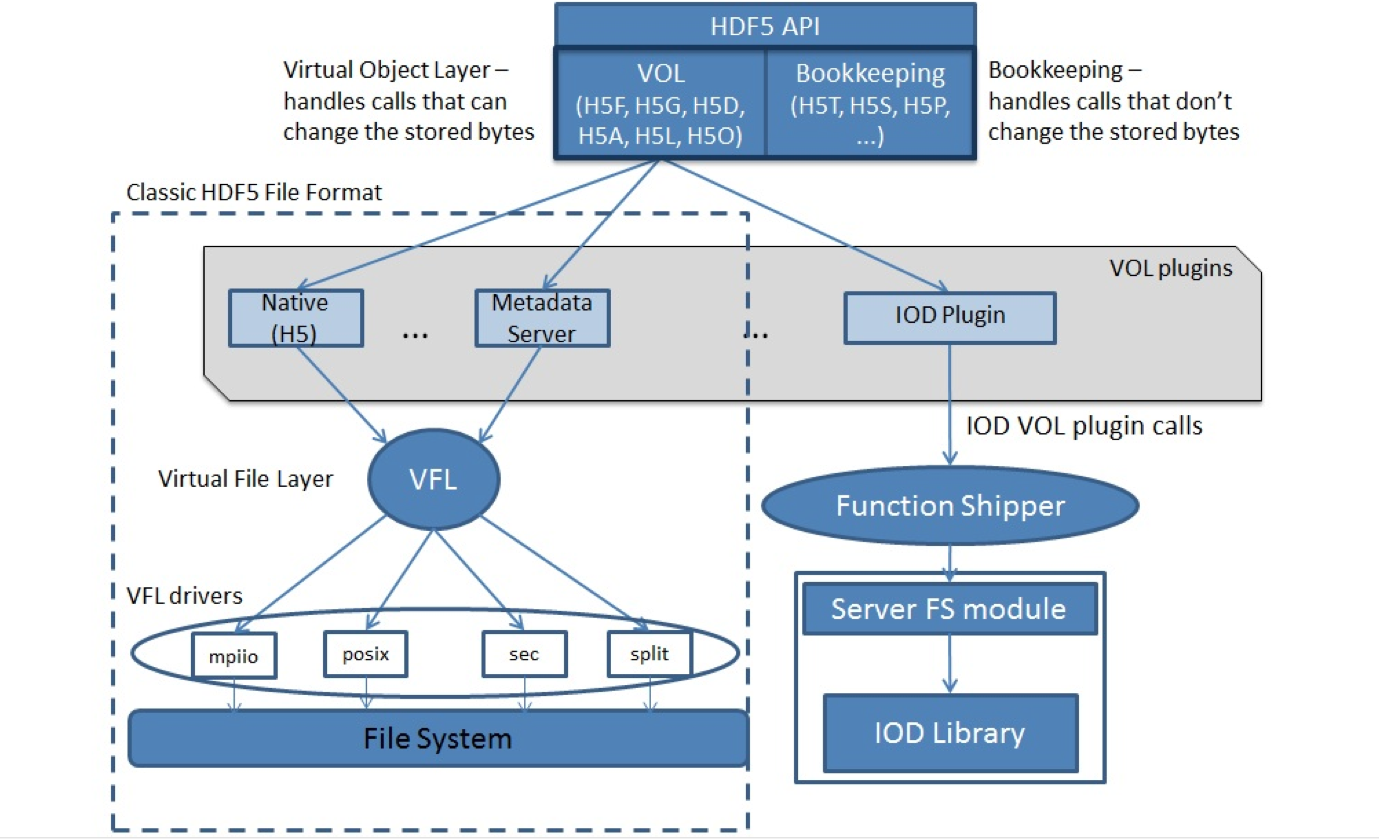
\includegraphics[scale=0.20]{images/vol-arch.png}
\caption{Architectural view of the VOL abstraction mechanism}
\label{fig:vol-arch}
\end{figure}

\subsection{IOD VOL plugin}
\label{iod-vol-plugin}

The IOD VOL plugin serves as the bridge between HDF5 and the IOD API (Figure \ref{fig:vol-arch}). The application calls the HDF5
library while running on the system's compute nodes. Using the VOL
architecture, the IOD VOL plugin uses a function shipper (RPC library)
to forward the VOL calls to a server component running on the I/O nodes
(IONs). At that point, the VOL calls are translated into I/O Dispatcher
(IOD) API calls and executed at the IONs.

The mapping between HDF5 objects and IOD objects is the following:

\begin{itemize}
\itemsep1pt\parskip0pt\parsep0pt
\item
  file = container
\item
  dataset = array
\item
  group = key-value store
\item
  attribute = key-value store
\end{itemize}

\section{IO Forwarding Layer}
\label{sec:iof}

The IO Forwarding layer offers a mechanism to reduce the concurrency impact of
the massive process count on the storage stack. A current trend mixing MPI with
a threading library like OpenMP is addressing the same issue. In this case,
the storage stack has far fewer end-points in which to receive requests and
data from compute processes. By reducing the number of simultaneous requests,
delays can be reduced. This has been demonstrated for the file open operation
with Lustre~\cite{lofstead:2009:adaptable} and to some degree for accessing the
storage devices themselves~\cite{lofstead:2010:io-variability}. The BlueGene
platform incorporated dedicated hardware to perform this role. The proposed
functionality for this layer has no special features beyond those previously
demonstrated.

\section{IO Dispatcher Layer}
\label{sec:iod}

The core idea for IOD is to provide a way to manage the IO load that is
separate from the compute nodes and the storage array. Communication intensive
activities, such as data rearrangement, can be moved to the IOD layer
offloading the communication load from the compute nodes. IOD has three main
purposes. First, if the optional burst buffer is available, it works as a fast
cache absorbing write operations for the slower trickle out to the central
storage array. It can also be used to retrieve objects from the central storage
array for more efficient read operations and offers data filtering to make
client reads more efficient.  Second, it offers the transaction mechanism for
controlling data set visibility and to manage faults that would prevent a data
set from being used. Third, data processing operations can be placed in the
IOD. These operations are intended to offer data rearrangement, filtering, and
similar operations prior to data reaching the central storage array.

While these ideas are not necessarily new, they are new twists on best of class
efforts for these technologies. For example, offloading the collective
two-phase data sieving from the compute nodes to reorganize data has proven
effective at reducing the total time for writing data due to fewer participants
involved in the communication patterns~\cite{lofstead:2011:nessie-staging}.
Beyond these broad items, there are many important details some of which are
examined in more detail below.

\subsection{I/O Dispatcher API}
\label{sec:fast-forwards-io-dispatcher-api}

The Fast Forward I/O and Storage project is aimed at integrating many of
the services existing currently in middleware libraries in a
next-generation storage stack, exposed through a non-POSIX,
transactional, asynchronous, object-based API.

From a high-level point of view, the Fast Forward's I/O Dispatcher (IOD)
interface allows the user to:

\begin{itemize}
\itemsep1pt\parskip0pt\parsep0pt
\item
  transactions
\item
  asynchrony
\item
  objects
\item
  layout
\item
  placement
\item
  formats
\end{itemize}

Type of objects:

\begin{itemize}
\itemsep1pt\parskip0pt\parsep0pt
\item
  container
\item
  key-value store
\item
  blobs
\item
  multi-dimensional arrays
\end{itemize}

As mentioned previously, IOD allows to store distinct types of objects.
From here on we will limit our discussion to multidimensional arrays
(HDF5 datasets) and leave the treatment of other object types as future
work. A multidimensional array can be sharded among the distinct I/O
nodes in the staging area. The IOD API supports the following
strategies:

\begin{itemize}
\itemsep1pt\parskip0pt\parsep0pt
\item
  \textbf{contiguous}. fixed chunking, distributed in a round-robin
  fashion accross the I/O nodes.
\item
  \textbf{chunked}. same as above but with irregular (sparse) chunking.
\item
  \textbf{user-defined}. either contiguous or chunked but user specifies
  where to place each individual shard.
\end{itemize}

It is possible to request the transformation of an object's physical
layout to other formats, having multiple copies of the same objects in
multiple formats if desired. Also, the user can pre-fetch objects from
the storage cluster into the I/O nodes or read them directly from the
storage cluster. At the semantic level (HDF5), indexes can be created
for datasets, which results in being able to read through an index
instead of directly from the base array.

All these distinct alternatives result in having many different ways of
executing the same analysis task. In the future, we plan to extend our
design to incorporate an optimization phase that will prepare a task by
taking into account the distinct possible ways of executing and select
the most promising one. In our subsequent discussions, we consider only
data-movement optimization, i.e., sending the analysis code as close as
possible to the data. In practice, this means we focus on identifying
sharding of datasets and execute code accordingly over the appropriate
shards.

\subsubsection{Sharding}
\label{sec:sharding}

The idea of sharding is to store a portion of a data set on a single storage
target. This is similiar in concept to the HDF-5 hyperslab. The FFSIO stack
supports sharding the data in the default or some other structured way as well
as ``re-sharding'' based on application needs. For example, reordering the
data so that a different dimension is the ``fast'' dimension may greatly
improve the performance of a subsequent data analytics task. A common scenario
where this is common is a Fortran code (column-major) writes data for a C code
(row-major) to analyze.

\subsection{I/O Nodes}
The ``I/O nodes'' handle requests forwarded by the scientific applications,
potentially integrate a tier of solid-state devices to absorb the burst of
random operations, and organize/re-format the data so that transfers to/from
the staging area from/to the traditional parallel file system can be done more
efficiently. It also has the capacity to executing analysis on the fresh data
that has just been generated by simulation applications running at the compute
nodes. As the data arrives, re-organization and data preparation can be applied
in order to anticipate the execution of analytical tasks.

\begin{figure}[htbp]
\centering
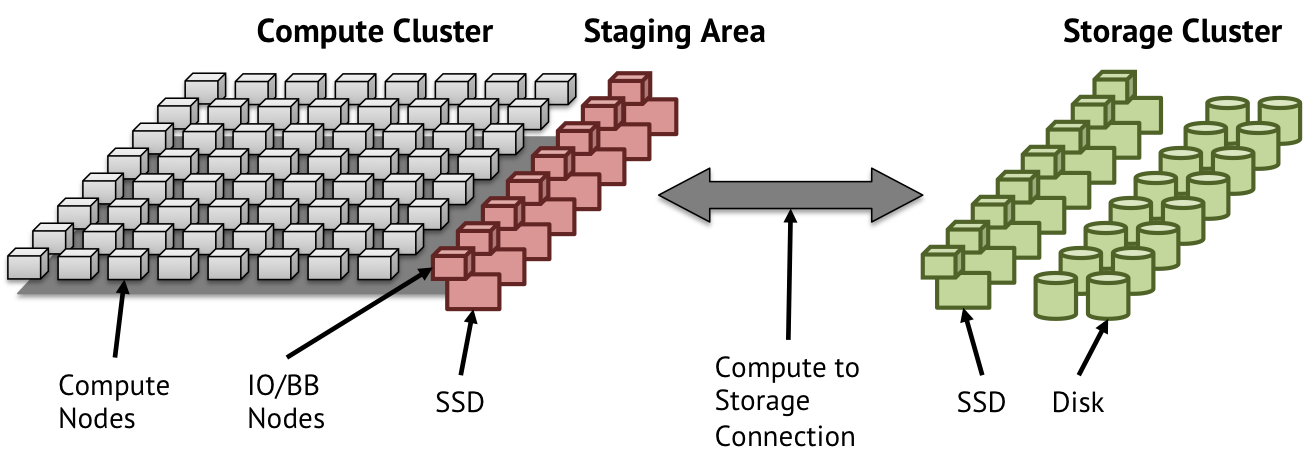
\includegraphics[scale=0.30]{images/exa-arch.png}
\caption{Exascale Architecture}
\label{fig:exa-arch}
\end{figure}

A common cluster configuration for this type of deployment is shown in
Figure~\ref{fig:exa-arch}. The designated I/O nodes (IONs) are connected to the
compute nodes (CNs) through the same fast fabric (e.g., InfiniBand), while the
connection to the external storage cluster is through a secondary slower
channel (e.g., 10Gb Ethernet). I/O staging thus introduces a new layer in the
application-to-storage stack, as shown in Figure~\ref{fig:exa-stack} (left).

%In current proposals, the stack is managed by middleware that sits between the
%application and the parallel file system. Since most of the applications assume
%a POSIX interface to storage, existing middleware either transparently handle
%the I/O operations, appearing as regular POSIX calls to applications; or modify
%the I/O API as little as possible in order to minimize the impact on production
%codes.
%
%As we move towards the exascale goal, this way of interfacing with storage
%becomes more of an obstacle. Many features provided by the stack are hidden by
%the middleware/POSIX layers. If these were visible to the applications, and if
%the applications were able to control how the underlying layers behave, they
%would benefit greatly since the domain knowledge that is available at the
%application level could be used to execute storage operations efficiently. One
%more implication of the 25-year-old POSIX API is in cumbersome middleware,
%since metadata has to be part of the same uni-dimensional byte array being
%stored.
%
%The Fast Forward Storage I/O project is aimed at merging the features of
%existing middleware into a next-generation parallel file system stack. This new
%storage API termed the I/O dispatcher (IOD) is object-based, transactional,
%asynchronous and I/O-staging-aware (Figure~\ref{fig:exa-stack} (right)).

\begin{figure}[htbp]
\centering
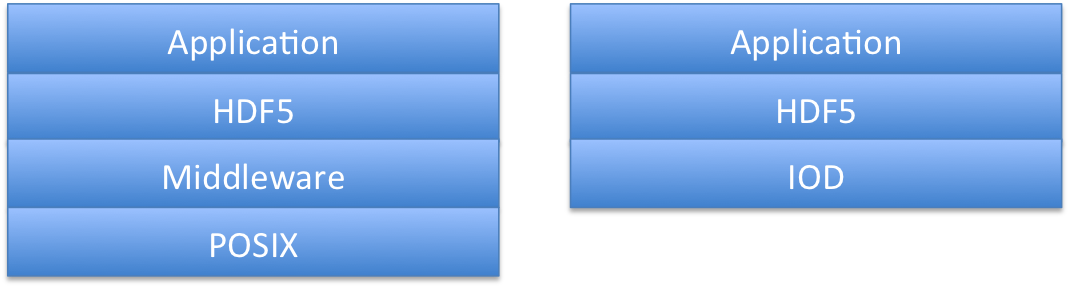
\includegraphics[scale=0.30]{images/exa-stack.png}
\caption{Top-to-bottom view of the component stack}
\label{fig:exa-stack}
\end{figure}

%The prototype stack, from a top-down point of view, has the following
%components:
%
%\begin{enumerate}
%\def\labelenumi{\arabic{enumi}.}
%\itemsep1pt\parskip0pt\parsep0pt
%\item
%  Arbitrarily Connected Graphs (ACG).
%\item
%  HDF5 extensions.
%\item
%  I/O Dispatcher (IOD).
%\item
%  Distributed Asynchronous Object Storage (DAOS).
%\item
%  Versioning Object Storage Device (VOSD).
%\end{enumerate}
%
%Applications running on the compute nodes will be written in Python scripts or
%in C++ using the HDF5 APIs. These applications will execute analysis on
%graph-based data (ACG). The point is to demonstrate both the HPC and BigData
%use cases of the Exascale architecture. The data structures will be stored in
%HDF5, for which new API extensions will be implemented. These new API calls
%will expose the transactional, asynchronous and function-forwarding semantics
%of the underlying stack.

As mentioned before, the stack provides \emph{non-POSIX, object-based,
transactional and asynchronous active-storage}, meaning that POSIX is
supplanted by new object interfaces that reach up to the HDF5 layer
(Application I/O in the stack diagram); transactional semantics are present,
from HDF down to the VOSD layer (Storage layer); clients don't need to wait for
any blocking operation; and analysis can be shipped and executed on I/O or DAOS
nodes.

\subsection{Burst Buffers}
\label{sec:burst}

The idea of burst buffers were initially explored in the context of data
staging~\cite{abbasi:2007:datatap,Abbasi:2009:datatap,nisar:2008:staging,zheng:2010:predata}.
These initial designs all use extra compute nodes to represent the data storage
buffer given the lack of any dedicated hardware support for this functionality.
The desired outcome of these initial studies is to motivate how such
functionality might be incorporated and the potential benefits.  Later, these
concepts were proposed to be incorporated as part of the IO
stack~\cite{nowoczynski:2008:zest,bent:2012:challenges,bent:2012:burst-buffer}.
The current Fast Forward IOD design recommends incorporating SSDs, but
specifically lists these devices as optional. Unfortunately, not incorporating
burst buffers and the use of SSDs in the IOD layer may be problematic.  First,
the IOD design currently is written assuming burst buffers. This means that the
bulk of IO operations will only hit the IOD layer and proposed functionality,
such as the function shipping, do not discuss the impact on the DAOS layer or
the operators themselves should a burst buffer not be available.  Consider the
important functionality of data rearrangement and doing things like changing
the fast array dimension on shared, spinning media.  The design of DAOS assumes
that it will only be involved when persisting a completed transaction and only
for a fraction of the total transactions created.  Transaction frequency at the
IOD layer can be higher since IOD does not ``flatten'' transactions. Flattening
is the process of transferring the set of copy-on-write changes from
transaction/epoch $n$ to transaction $n+m$ into the DAOS layer. The DAOS layer
mirrors the copy-on-write functionality, but stores the differences between
epochs rather than individual transactions. The primary difference is that at
the DAOS layer, data is stored in large, logically contiguous chunks to manage
the metadata load and hopefully improve read performance.

%One of the bigger concerns is the observation that the original data staging
%proposals all used compute nodes while the newer proposals seek not only to
%make them a fixed portion of the IO stack, but also shared across all machine
%users. The PreDatA~\cite{zheng:2010:predata} paper in particular examines the
%potential costs and advantages of where to place operators similar to the IOD
%proposed function shipping. There are two key takeaways from PreDatA. First,
%placement matters.  Depending on the communication intensity vs. computation
%intensity, where along the IO path to place the operation can matter
%significantly. Second, and more importantly, the amount of time spent
%processing for the operators was stretched to the point where it consumed
%nearly all of the time between IO operations. The given ratios of compute
%processes to staging process examined is representative for future extreme
%scale platforms. If anything, the ratios offer more staging processes than IOD
%processes would be available.
%
In the case of the written IOD design, it describes a fixed-sized staging area
that is partitioned on a per-application basis.
%This is unlikely to be useful
%because of the limited compute and communication capacity to spare to perform
%these operations at a bottleneck in the IO path.  The use of a separate data
%staging area intentionally separate from the IO path allows using operators on
%limited resources leaving the IO path clear for strictly data movement. A
%nuance of this design is discussed in the Design Philosophy below.
%
%By concentrating the Burst Buffers and function shipping into the storage
%stack, three problems arise.  First, the amount of network bandwidth, IO
%bandwidth, and compute power consumed for example operations from a single
%application is likely to completely monopolize the IOD processes. Second, if
%space and time partitioning is used instead, the functionality risks being too
%small to be useful. Third, the long-term hardware performance advantage for
%SSDs is questionable. Recent studies have shown that the erase-before-write
%and interference between reading and writing with flash-based SSDs can cause
%severe performance problems~\cite{skourtis:2013:ssd-performance}. The inclusion
%of an optional use SSD layer in the new Trinity machine at Los Alamos will
%offer a test bed to determine how likely these observed problems would affect a
%production extreme scale platform.
%
%Given these features, the optionality and even incorporation of burst buffers
%in the current design should be carefully considered. Much of the advanced, key
%functionality proposed as they are currently designed ultimately relies on the
%existence of burst buffers to work. Further thought about how to have an IOD
%layer both with and without a burst buffer is required before they can be
%considered optional. As the design stands today, they are a required part of
%the IOD layer for proper functioning. Unfortunately, it is not clear that they
%can address the performance concerns they are intended to cover.

\noindent\textbf{Design Philosophy}

The burst buffers design, as presented in the IOD documents, limits the
placement of the function operators and SSD buffers to the IO nodes. The team
does acknowledge the limitations of this design and intend to ultimately focus
on spreading the IOD layer from the IO nodes into the compute area as well.
This is intended both to help address the limitations of the IO bandwidth and
compute capability of these few nodes for data processing, but also to take
advantage of new layers in the storage hierarchy. By incorporating NVRAM into
compute nodes, new options for buffering data prior to being moved to
centralized storage become available and addresses some of the concerns about
SSD performance. For example, including a small amount of Phase Change memory
into many or most compute nodes offers a way to move data outside of both the
compute and IO path for data and communication intensive operations. Other 
projects~\cite{zheng:2010:predata} have suggested this will have value, but the
cost will have to be considered as part of the overall platform budget. This
lessens the impact of some operators while offering additional options for
places to store data.

Burst buffers being optional is a high level goal, but not one considered at a
detailed level within the design. For example, if there is no burst buffer, all
of the advanced functionality proposed for the IOD layer would have to work
against the DAOS layer instead. For example, function shipping assumes it will
operate on fast, local data within the IOD layer rather than against the
globally shared DAOS layer. With the additional desire to support using compute
node resources for these operations, serious work will be required to make a
fully functional end-to-end IOD layer implementation for a production system.

Another concern that is acknowledged, but no thought has been applied to, is
the requirement that a single IOD process of the set assigned to an application
is the master for any operation.  Should the number of concurrent applications
exceed the available nodes, sharing an IOD process will be required. The
requirements both in terms of scheduling and resource management were cut from
the project due to funding limitations. Since partitioning of the IOD processes
for exclusive use by particular applications is the assumed operating mode,
should insufficient IOD resources be available, either a job could be delayed
or IOD resources could be reallocated from a different process could be
redeployed for use by the new job. Handling resilience concerns for the IOD
processes must also be address.  These sorts of considerations still need to be
made for a full production system.

\section{DAOS Layer}
\label{sec:daos}

The Distributed Asynchronous Object Storage layer serves as the traditional
parallel file-system interface layer for the storage devices. This is the
consistent, global view of the underlying devices represented in this stack
by the VOSD layer.

This is the layer where the container/object model is translated into the
physical storage requirements dictated by the physical storage underneath (the
VOSD layer). The two key design elements of this layer are the handling of
epochs and the mapping of conatiners and objects to the underlying storage.

Epochs are represented throguh the shard mechanism. Each container shard is
versioned according to the transactions in the IOD layer that are persisted to
the DAOS layer as an epoch. The container shard is a piece of the container
with the contained objects concept. Since the container is largely logical,
this generally maps to a shard of an object within a container.

Each container is represented by a directory on some storage device containing
symbolic links to all of the shards it contains and maintains the epoch ID.
In particular the Highest Committed Epoch (HCE) is an important concept for
quickly identifying which version of a shard to retrieve and to block writes to
older epochs since those have been committed.

\section{VOSD Layer}\label{sec:vosd}
The Versioning Object Storage Device (OSD) layer operates as the layer for each
persistent storage device used to support the parallel storage array. In the
purest form, it uses a local file system to arrange storage of objects that
represent parts of the higher level objects in containers.

The base level implementation continues the space optimization of only storing
changes for new versions by using a copy-on-write file system. The prototype
uses ZFS~\cite{zhang:2010:zfs} for the known stability and integration with
Lustre. In a production version of the FFSIO stack,
btrfs~\cite{rodeh:2013:btrfs}, The Linux B-Tree File System, given its
open-source backing and GPL licensing, is a likely long-term choice.

At a more detailed level, the design for VOSD is an increment beyond the
current Lustre Object Storage Device design to incorporate the idea of shards
and the versioning aspects of transactions/epochs. For every DAOS shard, the
VOSD has information for storing and accessing the currently commited version,
the Highest Committed Epoch, as well as a staging dataset represeting the
next version of the object being stored. Both of these are combined in a shard
root.

For data integrity, an intent log is maiained as part of the underlying file
system enabling fault recovery.

Beyond the functionality to incorporate and expose the copy-on-write nature
of the underlying file system and the semantics for storing and processing
shards and their associated epochs, this is largely an evolution of the
existing Lustre OSD layer.

\section{Broader Design}
\label{sec:broader}

%At a broader level, there are some concerns that were partially clarified
%through conversations with the team.  Consider a shared file system across an
%HPC data center. The current design maintains the metadata in its own
%container. Since copying data from the IOD layer to the DAOS layer requires an
%explicit persist call, how and when synchronizing the metadata across the
%layers and potentially across machines occurs is undefined. Delaying
%synchronization until an explicit persist is called will reduce the update
%frequency, but delays the data visibility on other platforms. Ideally, the
%metadata object would need to be automatically persisted every time a container
%transaction is persisted to the DAOS layer.
%
%The implication of this is that every transaction persist is double operation
%to account for the metadata persist. More importantly, the IOD-layer version of
%the metadata container may contain readable transactions that have not been
%persisted to the DAOS layer. How to handle this inconsistency between the two
%layers still needs to be explored.
%
A point of confusion rather than a potential design challenge is the change in
definitions between the IOD layer and the DAOS layer.  For the IOD layer, a
container is a collection of objects. For the DAOS layer, a container is a
collection of objects across a set of shards. For the IOD an object may be a
shard of a global array.  For DAOS, a shard can host a set of DAOS objects.
Having the same names with locally correct, globally conflicting definitions
serves to confuse how the system should work.

\subsection{Transactions and Epochs}
\label{sec:transactions}

The transaction mechanism manifests in two forms. At the IOD layer, they are
called transactions and are used to judge whether or not a set of distributed,
asynchronous modifications across a set of related objects is complete or not.
It is also used to control access by treating the transaction ID of committed
transaction as a version identifier.  At the DAOS layer, they are called epochs
and represent persisted (durable) transactions from the IOD layer. Each of
these offers different functionality, but are connected as is explained below.
%How these differ from the \DDT approach is also explored.  While IOD's and
%\DDTns's transactions are seemingly very different, they use a similar
%high-level design, but very different implementation, to solve the same
%problem.

\subsubsection{IOD Transactions}
To understand how transactions are used in the IOD layer, some terminology and
concepts must be explained first. At the coarsest grain level is a container.
Each container provides the single access context through which to access a
collection of objects. Transactions are the way that a series of modifications
to the objects within a container are treated atomically. Conceptually,
containers corresponds to a something akin to an HDF5 file in a traditional
file system. The objects in each container represent different data within a
file.  The three initially defined object types are key-value stores,
multi-dimensional arrays, and blobs.  The easiest way to understand these types
is to evaluate these from the perspective of an HDF-5 file, the initial user
interface layer. The key-value store represents a collection of attributes or
groups. The array represents a potentially multi-dimensional array.  The blob
represents a byte stream of arbitrary contents.  The fundamental difference
between an array and a blob is that the array has metadata specifying the
dimension(s). At the physical layer within the IO nodes, all of these objects
may be striped across multiple IO nodes.  Given this context, the transactions
come in two forms.

First is a single leader transaction where the IOD manages based on calls from
a single client. The underlying assumption is that the client side will manage
the transactional operations itself and the single client is capable of
reporting to the IOD how to evolve the transaction state. 

The second form is called multi-leader and has the IOD layer manage the
transactions. In this case, when the transaction is created, a count of clients
is provided to the IOD layer. As clients commit their changes to the container,
the reference count is reduced. Once the count reaches 0, the transaction is
automatically committed.

\noindent\textbf{Design Philosophy}

Undocumented, but inherent in the design of these transactions is how faults
are detected. The initial design assumes the current Lustre fault detection
mechanism that can determine if a process or node is no longer reachable. This
detection happens at the DAOS layer and when a fault is detected, the rollback
process is pushed up to the IOD layer for all non-persisted or non-committed
transactions. This defines how a fault will be detected and what will trigger a
passive fault recovery (i.e., transaction abort).

There are two steps for beginning a transaction on a container. The first step
is for one or more process to open the container. This handle can be shared
eliminating the need for every participating process to hit the IOD layer to
open the file. The second step is a call to determine how many leaders will
participate in the transaction. In the single leader case, there is no
aggregation of success/fail statuses to determine the final transaction state.
Instead, it is assumed that the client will fully manage the transaction. In
the multi-leader model, some subset from 2 to $n$ where $n$ is the count of all
processes, declare themselves a leader for this container operation to the IOD
layer. Any number of processes can participate in modifying container without
regard to whether or not they are a leader. Once each leader has finished, with
the assumption that any clients they may be responsible for are finished as
well, the IOD layer aggregates those responses to either commit or abort the
transaction.

Ultimately, with the passive detection of faults for transaction leaders, the
transaction mechanism can work very well. A mostly unstated restriction that is
being relaxed is that every sequential transaction on a container is considered
dependent on the earlier transaction. Should one output be delayed and the
subsequent five succeed, when the delayed process finally fails, all six
transactions are rolled back. The thought of using this mechanism to store
subsequent checkpoint outputs in the same container to both save space, but not
care if one fails, cannot work in the current form. This has been acknowledged
and is being relaxed requiring a new parameter to the creation of a transaction
determining if it will be dependent or not.

\subsubsection{DAOS Epochs}
The Epoch mechanism differs from transactions. Instead of focusing on when a
particular output is complete, an epoch represents incremental persisted copies
of a container. To simplify the mapping between an IOD transaction and the DAOS
epochs, when an IOD transaction is persisted to DAOS, the IOD transaction ID is
the used as the epoch ID. The key difference is that at the DAOS layer, some
transaction (epoch) IDs will not be represented since not all IOD transactions
are necessarily persisted.

\subsection{Metadata Management}
Metadata management has been a perennial challenge for parallel storage
systems.  Eliminating metadata management as a special case and instead
treating it just as data is a central design goal of the Fast Forward project.
This is a hybrid approach to metadata management that is half-way between
providing no inherent metadata support and having a fully integrated, but
separate metadata management system.

Eliminating metadata as a core component of a file system is not new. It has
been explored as part of the Light Weight File Systems
project~\cite{oldfield:lwfs}. In LWFS, the metadata service is explicitly
limited to a user task with the storage layer limited to data
storage/retrieval, authorization, and authentication. This approach proved
workable. Using this hybrid approach is less common~\cite{weil:2006:ceph} and
introduces other issues.

IOD and DAOS both share a philosophy that they will have to maintain the
metadata about how the physical pieces of the logical objects are striped and
where they are placed. The primary metadata management is done at the DAOS
layer with the IOD layer relying on the DAOS layer for all authoritative
information about containers and objects. The only place where the IOD layer
manages metadata for itself is to manage how the different objects are striped
across the IO nodes.

\noindent\textbf{Design Philosophy}

While the metadata design is not fully defined, there are a few things that
are intended. For example, there is a standard, well-known container that is
the system metadata. This includes the list of all other containers. This
container is treated like any other data in the system and striped as
appropriate. Unfortunately, this still couples the metadata to a single object
that must serialize access. If the metadata, including information about
striping and other data layout operations were separated completely from the
data path, more scalable throughput could be achieved. The real challenge of
this is introduced by the IOD, DAOS, and VOSD layers collectively. Each of
these requires some different metadata storage and the migration is transparent
to the user.  Supporting fully independent metadata with this model is
difficult. Serious thought on how to do this effectively outside the data path
should be considered for phase two.

%Based on the lessons from the \DDT metadata
%service~\cite{lofstead:2012:txn-metadata} construction and the prior
%experiments with LWFS, having a completely separate metadata service is
%workable. Rather than making it a bottleneck in the IO path, it is another
%service that users must interact with if they need those services.  Users can
%manage everything by maintaining the metadata including the list of objects
%themselves. However, there are drawbacks to this 100\% client-side approach.
%
%With a client-side only approach, there is a serious risk of the metadata
%service and the object store getting out of sync.  While having a metadata-less
%object storage service is desirable, the different semantics from traditional
%file systems requires some considerations. In this case, should these services
%get out of sync, three particular risks are introduced.  First, a client could
%create a dangling entry in the metadata service that does not correspond to any
%objects in the object store. Second, a client could create orphaned objects
%that have no associated metadata entries. Third, updates to the metadata or
%object store service should be an atomic operation, but due to a lack of
%coordination, a window where the system is inconsistent appears.
%
%Ultimately, the consistency semantics required must be determined. If a
%metadata service is required and it must be in sync with the object storage
%service, then additional work must be performed. In traditional file systems,
%the metadata and object storage updates are atomic. With decoupling metadata
%from object storage, should this atomicity still be desired, it requires both
%the ability for the services to participate in a task that is part of a larger
%atomic operation and a higher-level mechanism to manage the atomic operation.
%
%Overall, while additional work is required to maintain a client-side only
%metadata service, it eliminates any potential bottlenecks related to updating
%metadata related to the object storage. The burden of tracking striping and
%other metadata that has traditionally been part of the metadata associated with
%the file system will have to be maintained by the object storage service. The
%lack of a centralized, serialized bottleneck to store that information improves
%concurrency.

%\subsection{Comparison to \DDTns}
%The \DDT project~\cite{lofstead:2012:txn} sought to develop an efficient
%approach for handling ACID-style transactions in an environment with parallel
%clients and multiple servers (doubly distributed). Rather than being aimed
%solely at data movement operations, \DDT seeks to address the general problem
%of managing any operation with multiple clients and servers.  Consider the
%management of the analysis/visualization area, potentially similar to the IOD
%concept. The transaction protocol is used to help manage resizing of the
%resource allocation to the various analysis and visualization components.  For
%the purposes of this discussion, \DDT could also be used to manage changing how
%IOD processes and/or nodes are used without exposing these changes to the
%client processes prematurely.  This has been described and analyzed
%previously~\cite{dayal:2013:io-containers}.
%
%The example metadata and data storage services created as part of the \DDT
%project have no dependencies between transactions that prevent visibility
%should an older version be incomplete. This additional, intentional requirement
%by IOD offers different functionality than \DDTns's example services. In the
%case of \DDTns, the functionality is more minimal, but also avoids some of the
%concerns outlined below.
%
%The second iteration of the protocol~\cite{lofstead:2013:pdsw-txn} fixed
%scalability issues and demonstrated a scalable client-side coordination model
%with excellent performance. The performance measured for a complex transaction
%with \DDT is illustrated in Figure~\ref{fig:performance}. This performance is
%explored in detail in a previous paper~\cite{lofstead:2013:pdsw-txn}.
%
%\begin{figure}[ht]
%%\vspace{-0.15in}
%\centering
%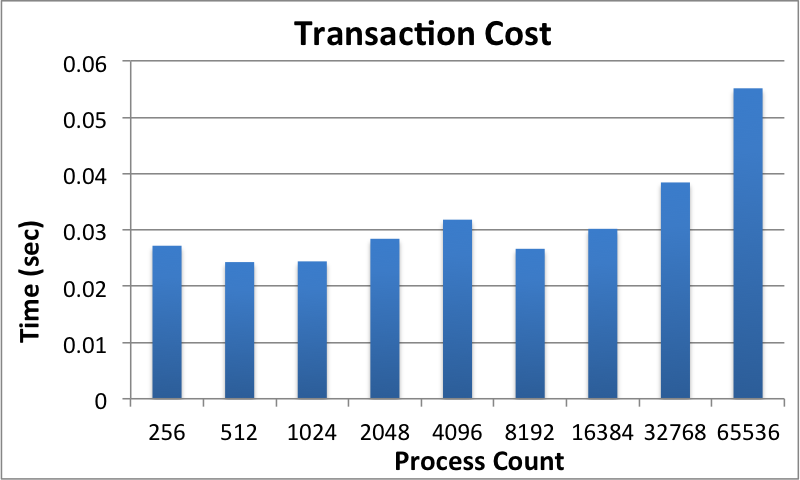
\includegraphics[keepaspectratio=true, width=0.9\columnwidth]{images/performance}
%\vspace{-0.15in}
%\caption{Total Transaction Overhead}
%\label{fig:performance}
%%\vspace{-0.15in}
%\end{figure}
%
%At a high level, both \DDT and the IOD transactions have the same design. In
%both cases, a hierarchical model is employed. In the case of \DDTns, it is a
%purely client-side tree using semi-synchronous messaging. The messaging itself,
%in the current implementation, uses asynchronous MPI messages. The synchronous
%component comes from the timeout mechanism used to detect faults.  It forces a
%level of coordination and synchronization for the protocol. For IOD, it is a
%server-side tree and fully asynchronous relying on the existing Lustre fault
%detection mechanism for failure detection. In both cases, there is a master in
%charge of managing the transaction and a collection of workers that aggregate
%into the master through second-level leaders. Beyond that, there are some
%significant differences. Some of the different choices made by IOD raise some
%possible concern.
%
%The multi-leader model introduces the possibility of forcing a rollback of an
%entire transaction when a partial retry might be sufficient for success. Since
%the transactions are managed at a high level rather than the individual
%tasks, a failure in a limited distributed task can cause the entire transaction
%to fail. For example, consider 10 processes each have 5 tasks, but 3 of those
%10 have an additional shared task to complete. If the task shared by the 3
%processes fails on any of the three, the entire transaction would roll back
%because it is a coarse-grained success/failure. If a concept like
%sub-transactions at a task granularity were used, then it would be possible for
%the one process that failed to report just that failure. Then the transaction
%manager could reassign the resources for these 3 processes and try just that
%operation again. If it now succeeds, then the overall transaction can be marked
%successful only redoing the minimum amount of work required.
%
%\begin{figure}[ht]
%\centering
%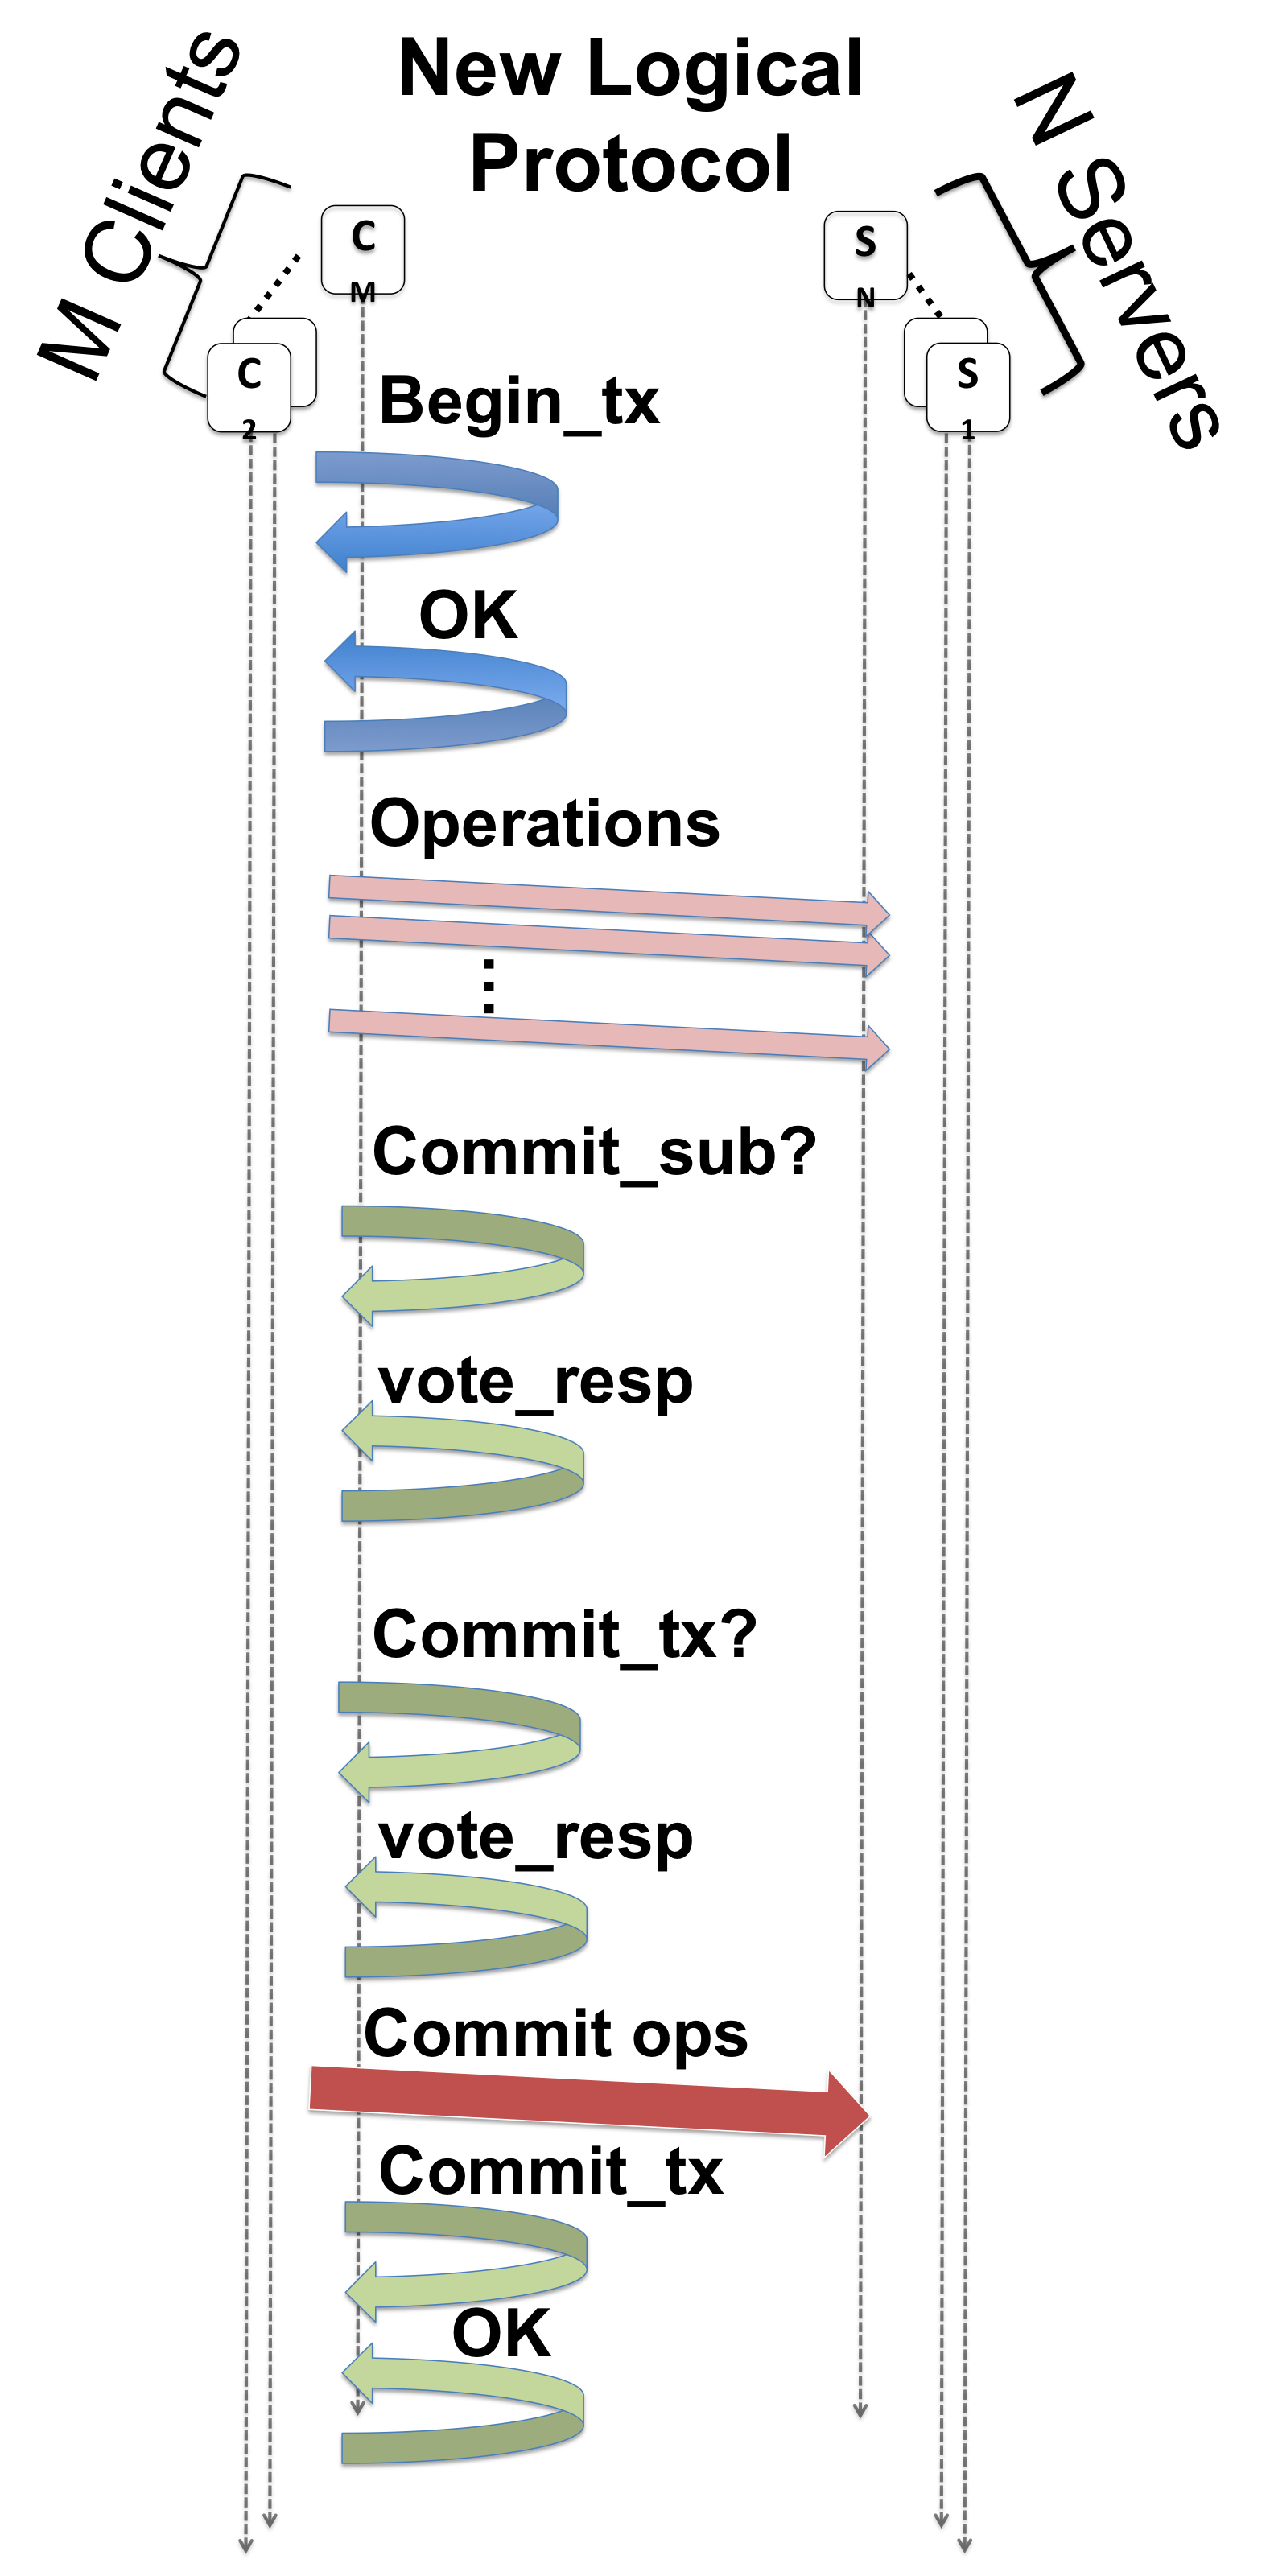
\includegraphics[keepaspectratio=true, width=0.5\columnwidth]{images/optimized-protocol}
%\vspace{-0.15in}
%\caption{Optimized Protocol}
%\label{fig:optimized-protocol}
%%\vspace{-0.25in}
%\end{figure}
%
%\DDT has addressed theses issues in a couple of ways. First, the
%sub-coordinators each have a list of processes from which they expect messages.
%Should a message be missed, it is noticed and corrective action can be taken.
%Second, \DDT has the concept of sub-transactions. The messaging requirements
%are illustrated in Figure~\ref{fig:optimized-protocol}.  Sub-transactions
%represent finer grained operations than the entire output, \DDT can manage
%multiple writes per client by using a sub-transaction to represent the output
%for any item to the file (container). Because of how the sub-transactions are
%managed, the singleton sub-transactions, ones in which only a single process
%participates, must be declared before the transaction begins so that its
%existence can be broadcast as part of the begin transaction message. This
%ensures there is global knowledge that the sub-transaction is expected.  That
%way if the coordinator (transaction leader) fails, whichever process takes over
%that role knows to expect a completion message for that sub-transaction or the
%overall transaction cannot complete. Global sub-transactions can be defined at
%any time since they are a global, synchronized operation broadcasting their
%existence. While this additional layer does introduce messaging, the overhead
%is quite small.
%
%The advantages of eliminating these messages is not performance as demonstrated
%by the performance of \DDTns. Instead, it offers a much less synchronous model
%that matches with different programming models, such as Charm++ or other
%task-based approaches. Since it can work for the bulk-synchronous model also,
%it is a more broadly applicable approach. This assumes that the observed
%potential issues can be addressed successfully.

\subsection{Function and Analysis Shipping}
\label{sec:fn-shipping}

In terms of the CN-ION communication model, a client/server architecture
is implemented: every ION runs an IOFSL (I/O Function Shipping
Layer) server; the IOFSL client is integrated into the HDF5
library which runs on each CN. A client can forward requests to any
number of IONs. Every I/O operation issued by HDF5 is asynchronously
shipped to the IOFSL server and asynchronously executed.

\subsection{ACG}
\label{sec:acg}

This will exemplify how applications make use of the Exascale stack. For
FF, support for
GraphLab 
and GraphBuilder will be prototyped, which are graph-processing
frameworks. GraphBuilder is a set of MapReduce tasks that extract,
normalize, partition and serialize a graph out of unstructured data, and
writes graph-specific formats into HDFS. These files are later consumed
by GraphLab, a vertex-centric, asynchronous execution engine that runs
directly on top of HDFS (i.e., non-MapReduce). The following illustrates
the architecture of both frameworks:

\begin{figure}[htbp]
\centering
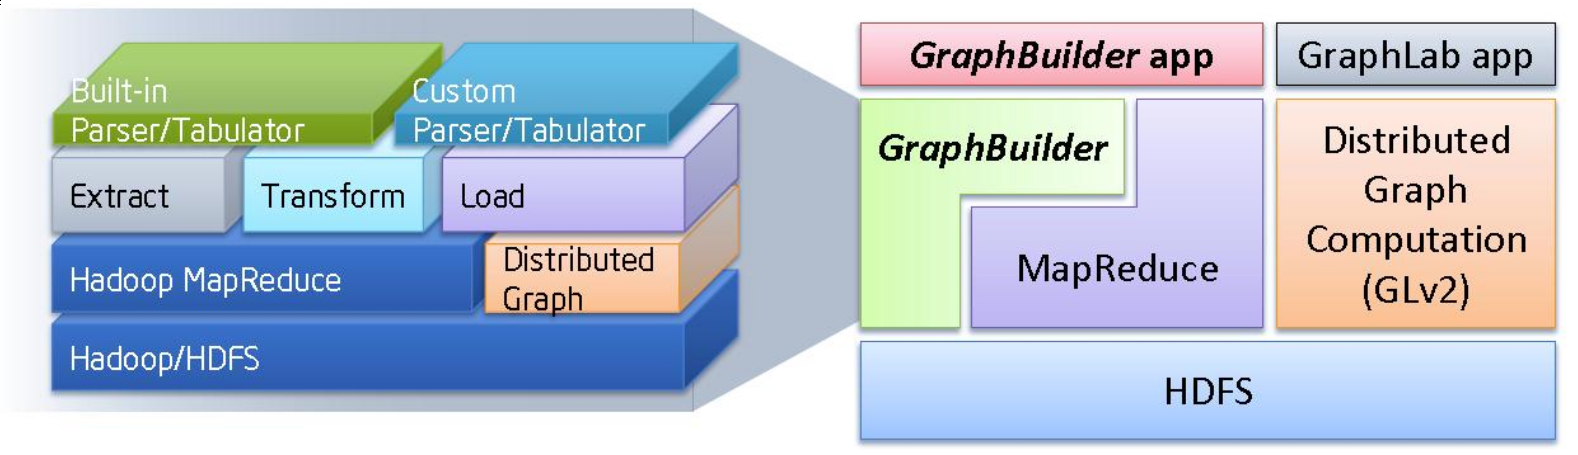
\includegraphics[scale=0.15]{images/graphlab-and-graphbuilder.png}
\caption{GraphLab and GraphBuilder stacks}
\label{fig:graphlab-graphbuilder}
\end{figure}

In order to make both work on top of the exascale stack, both have to be
modified. After these modifications are implemented, GraphBuilder will
be able to write the partitioned graph in (the newly proposed) HDF5
files which will thus be stored in the IOD nodes (or IONs) in a
parallel-optimized way. On the GraphLab side, HDF5-awareness will allow
the library to perform at high speeds by benefiting from the new
features (see next section). In general both frameworks will be modified
so that calls to HDFS-based formats are replaced by the proposed HDF5
ones. This is referred to as the HDF Adaptation Layer or HAL and will
provide, from the GraphBuilder/GraphLab point of view:

\begin{itemize}
\itemsep1pt\parskip0pt\parsep0pt
\item
  capability for storing the newly proposed HDF5 format
\item
  association of network information to vertices/edges
\item
  shipping computation to the IONs
\item
  asynchronous vertex updates
\item
  efficient data sharing ammong CNs
\item
  computation over versioned datasets
\end{itemize}

\section{Demonstration}
This stack has a prototype implementation intended to test concepts rather
than performance and scalability. It has focused on examining the interaction
of the different APIs for each layer to flesh out any detailed requirements
or concerns that may have been missed in the conceptualization of this IO stack.

We run this demonstration using two different modes. A standard HDF-5 test
application is used with the native file system layer writing directly to
storage is measured. Then, the same test is run against the requirements
prototype to demonstrate that it can function for this example as well. The
performance of both of these tests are reported to give a very rough idea of
the overhead that might be involved. Rather than a true overhead, this should
be considered the maximum overhead that should be expected once an optimized,
fully functional IO stack is deployed without relying on translating to an
underlying parallel file system. Figure~\ref{fig:evaluation} shows the
relative performance for both test runs.

The testing evironment for this demonstration is ....

\begin{figure}[htbp]
\centering
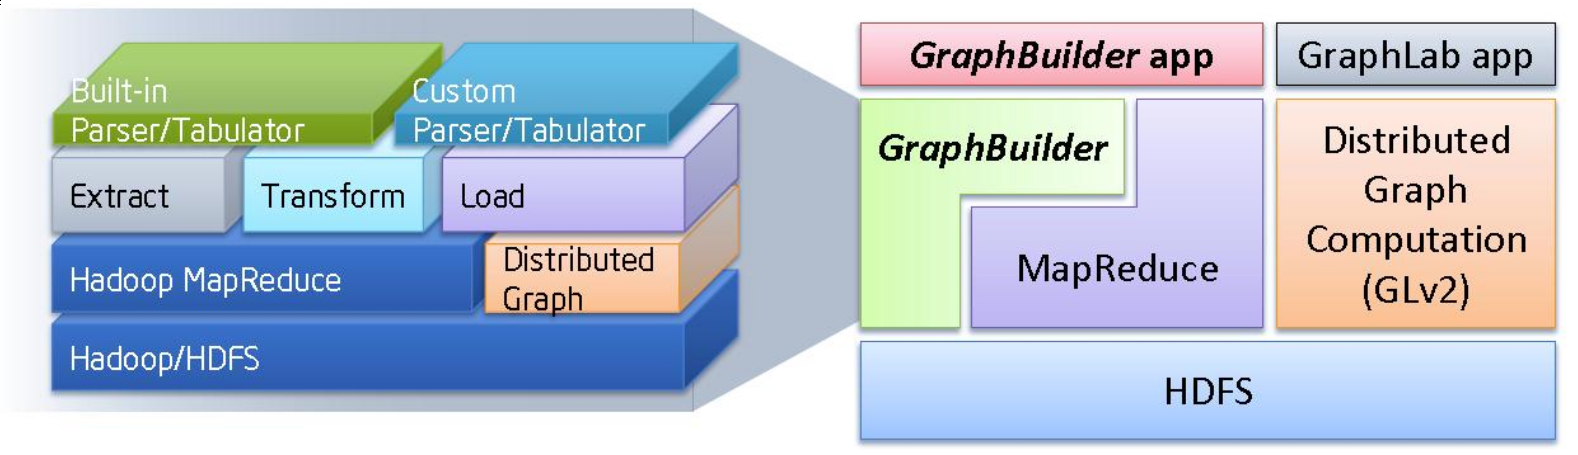
\includegraphics[width=\columnwidth]{images/graphlab-and-graphbuilder.png}
\caption{Functionality Demonstration Validation}
\label{fig:evaluation}
\end{figure}

\section{Conclusions}
\label{sec:conclusion}

The Fast Forward Storage and IO Stack project has designed a good first pass at
addressing the requirements for an extreme scale data storage mechanism. The
split between the IOD layer and the DAOS layer offers a fast place for
intermediate data without requiring the overhead of writing to persistent
storage. The envisioned transaction mechanism, while not perfect in the current
form, is another good attempt to address both failures and prevent access to
incomplete or incorrect data by downstream data consumers. Integrated with the
IOD functionality, this concept represents the consensus approach for what will
be required.

The partial metadata management incorporated into the IOD layer and the lack of
consideration for how to handle and recover from failures are oversights in the
current documents. It is our understanding that these will be addressed in the
next phase and we hope to help inform that effort with our experiences.

We hope that the efforts made in the \DDTns, Lightweight File Systems, and
other efforts to explore the requirements for this space, along with the
analysis presented in this paper will prove useful for the next phase of the
Fast Forward project.

\section{Acknowledgements}
The authors would like to thank Eric Barton, John Bent, Gary Grider, and
Quincey Koziol for their early review comments and discussions that clarified
the details of the design, the intent of the design, and the future plans.


\includegraphics[scale=0.07]{logos/doe_logo}

\includegraphics[scale=0.30]{logos/snl_logo}

\includegraphics[scale=0.35]{logos/nnsa_logo}
Sandia National Laboratories is a multi-program laboratory managed and operated
by Sandia Corporation, a wholly owned subsidiary of Lockheed Martin
Corporation, for the U.S. Department of Energy's National Nuclear Security
Administration under contract DE-AC04-94AL85000.

\bibliographystyle{abbrv}
\bibliography{paper}

\vfill\eject

\end{document}
